\documentclass[twocolumn, 12pt]{article}
\usepackage[utf8]{inputenc}
\usepackage{amsmath}
\usepackage{marvosym}
\usepackage{textcomp}
\usepackage{geometry}
\usepackage{array}
\usepackage{wrapfig}
\usepackage{multirow}
\usepackage{graphicx}
\usepackage{float}
\usepackage{wrapfig}
\usepackage{caption}
\usepackage{amssymb}
\usepackage[normalem]{ulem}
\usepackage{comment} % allows block comments

\geometry{a4paper, margin=.75in}



\begin{document}
\small
\section*{Controls and Dynamics}

%
\subsection*{Modelling}
\subsubsection*{Procedure}
\begin{figure}[h]
    \centering
    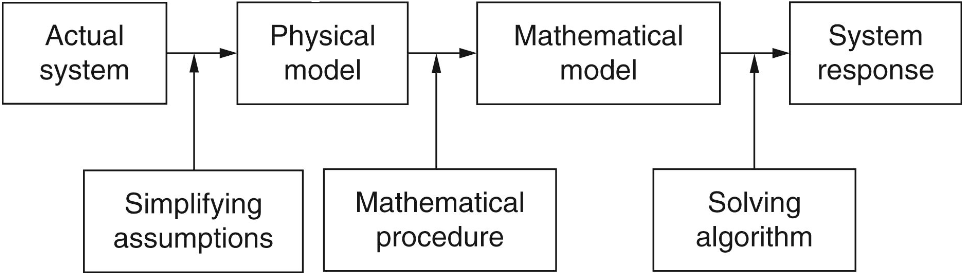
\includegraphics[width=0.45\textwidth]{Modelling Procedure.png}
    %\caption{Caption}
    \label{fig:Modelling Procedure}
\end{figure}



%
\subsubsection*{Elements and Equations}
\begin{equation*}
    e_m = k_e\omega \hspace{15pt} T_m = k_tl
\end{equation*}
\begin{equation*}
    T_{\text{stall}} = T_a|_{\omega=0, \hspace{3pt}\dot{\omega}=0} \hspace{15pt} \omega_0 = \omega|_{T_a=0, \hspace{3pt} \dot{\omega}=0}
\end{equation*}




%
\begin{comment}
\subsection*{Element Assumptions}
\underline{Translational/Rotational Mechanical}
\begin{itemize}
    \item Stiffness
    \begin{itemize}
        \item Massless element
        \item No friction
        \item Uni-directional motion
        \item Time-invariant
        \item \(x_i/\theta_i = 0\) at equilibrium
    \end{itemize}
    \item Friction
    \begin{itemize}
        \item Massless element
        \item No stiffness
        \item Uni-directional motion
        \item Time-invariant
    \end{itemize}
    \item Mass
    \begin{itemize}
        \item Point mass
        \item Uni-directional motion
        \item Time-invariant
    \end{itemize}
\end{itemize}
\end{comment}


%
\subsubsection*{Extended FBD Method}
\begin{enumerate}
    \item Divide physical model into ideal elements
    \item Assign force and displacement references
    \item Model single elements using assigned references
    \item Model the interactions between the elements using D'Alembert Law
        \begin{equation*}
            \Sigma \textbf{F}_{\text{ext}} - M\frac{d\textbf{v}}{dt}=0
        \end{equation*}
        \begin{equation*}
            \textbf{F}_m = M\Ddot{x} \hspace{10pt}\uparrow\downarrow\text{ to positive disp.}
        \end{equation*}
    \item Substitute element equations into D'Alembert Law equation(s)
    \item Algebrate equations into standard form
\end{enumerate}



%
\subsection*{Electrical Systems}
\begin{enumerate}
    \item Assign current and voltage references to each element
    \item Identify loops and nodes
    \item Model single elements using assigned refernces
    \item Use KCL, and KVL on loops and nodes
    \item Combine equations towards ODE(s)
\end{enumerate}



%
\subsection*{State Space}
\begin{enumerate}
    \item Define state space variables vector \textbf{q}. Pick variables that deal with energy, such as:
    \begin{itemize}
        \item \(x/\theta\) - potential energy
        \item \(v/\omega\) - kinetic energy
        \item \(e_c\)  - energy in a capacitor
        \item \(l_L\)   - energy in an inductor
    \end{itemize}
    \item Apply the derivative, and form the following equations:
    \begin{equation*}
        \dot{\textbf{q}} = A\textbf{q} + B\textbf{u}
    \end{equation*}
    \begin{equation*}
        \textbf{y} = C\textbf{q}+D\textbf{u}
    \end{equation*}
    Where:
    \begin{itemize}

        \item \(A, B, C, D\) are matrices
        \item \textbf{u} is the input forces vector
        \item \textbf{y} is some force in the system (i.e. force on a wall)
    \end{itemize}
    \item Solve using numeric solver (MATLAB/Simulink)
\end{enumerate}






% 
\subsection*{ODE General Forms}
\begin{equation*}
    \dot{x}(t) +\frac{1}{\tau}x(t) = \kappa u(t)
\end{equation*}
Where:
\begin{itemize}
    \item \(\tau\) is the time constant
    \item \(\kappa\) is the (input) sensitivity
\end{itemize}
\hline
\vspace{8pt}
\begin{equation*}
    \Ddot{x}(t) +2\zeta \omega_n \dot{x}(t) + \omega_n^2x(t) = \kappa \omega_n^2 u(t)
\end{equation*}
Where:
\begin{itemize}
    \item \(\zeta\) is the damping ratio
    \item \(\omega_n\) is the natural frequency
\end{itemize}
\hline


%
\subsection*{Laplace Land}
\begin{align*}
    s_{1,2} &= -\zeta\omega_n \pm \omega_n \sqrt{\zeta^2 -1}\\
            &= \alpha \pm \beta
\end{align*}
\begin{equation*}
    \tau = -\frac{1}{\alpha} \hspace{15pt} T_s =4\tau \hspace{15pt}  T_{\text{peak}} = \frac{\pi}{\beta} \hspace{15pt} O.S. = \exp{\frac{\pi \alpha}{\beta}}
\end{equation*}


\begin{itemize}
    \item Overdamped (\(\zeta > 1\)) 
    \begin{equation*}
        PFE \longrightarrow\frac{A}{s} + \frac{B}{s-s_1} + \frac{C}{s-s_2}
    \end{equation*}
    \item Critically Damped (\(\zeta =1\))
    \begin{equation*}
        PFE \longrightarrow \frac{A}{s} + \frac{B}{(s-s_1)^2} + \frac{C}{s-s_1}
    \end{equation*}
    \item Underdamped (\(0<\zeta <1\))
    \begin{equation*}
        PFE \longrightarrow \frac{A}{s} + \frac{Bs+C}{(s-\alpha)^2+\beta^2}
    \end{equation*}
    \item No damping (\(\zeta =0\))
    \
\end{itemize}




%
\subsection*{Linearization}
Taylor series approximation:
\begin{equation*}
    f(x)|_{x=\Bar{x}} = f(x)|_{x=\Bar{x}} + \left \frac{\partial f(x)}{\partial x} \right|_{x=\Bar{x}} (x-\Bar{x})
\end{equation*}



% 
\subsection*{Controls}
\begin{equation*}
    y_{ss} = \lim_{t\rightarrow \infty} y(t) = \lim_{s\rightarrow \infty}sY(s)
\end{equation*}
\begin{equation*}
    G(s) =\frac{Y(s)}{U(S)} \hspace{15pt}  G(s)_{\text{closed}} =\frac{G(s)_{\text{open}}}{1+ G(s)_{\text{open}}}    
\end{equation*}
\subsubsection*{Controllers}
\begin{center}
    \begin{tabular}{l c l}
        P  & &\(C(s)=k_p\) \\
        PD & &\(C(s)=k(s-z_0)\)\\
        PI & &\(C(s)=k\frac{(s-z_0)}{s}\)\\
        PID & &\(C(s)=k\frac{(s-z_0)(s-z_1)}{s}\)\\
    \end{tabular}
\end{center}
\subsubsection*{Root Locus}
\begin{enumerate}
    \item RL begins at the poles of the O.L.T.F. and ends at the holes of the O.L.T.F.
    \item The \# of poles = the \# of branches. Every pole moves towards a zero (finite or infinite)
    \item RL is symmetric about the real-axis
    \item Left of odd poles/holes. Moving right to left, count the real-axis poles and holes the RL exists to the left of odd numbered entries
    \item Asymptotes
        \begin{equation*}
            \#A = \#_{\text{finite poles}} - \#_{\text{finite zeros}}
        \end{equation*}
        \begin{equation*}
          \sigma_A = \frac{\Sigma s_i-\Sigma z_j}{\#A} \hspace{15pt} \theta_{A_i}= \frac{(2m+1)\pi}{\#A}
        \end{equation*} 
        \begin{equation*}
           m = 0,1,2,... (\#A-1)
        \end{equation*}
    \item Break away/in points
        \begin{enumerate}
            \item Find the O.L.T.F., then the char. eq.
            \item Solve for k
            \item Set \(s=\alpha \pm \ulem{j0}\), find \(k(\alpha) =eq.\)
            \item Find alpha value(s) that satisfy \(\frac{\partial k}{\partial\alpha}
            = 0\)
            \item Check them!
        \end{enumerate}
    \item Stability-Instability points
        \begin{enumerate}
            \item Find the O.L.T.F., then the char. eq.
            \item Input \(s=0\pm j\beta\)
            \item Solve the Re, Im parts, achieve k value(s)
            \item Check them!
        \end{enumerate}
\end{enumerate}

\end{document}
